\documentclass[12pt]{article}
%\usepackage[utf8]{inputenc}
%\documentclass[UTF8]{ctexart}
%\usepackage[UTF8, heading = false, scheme = plain]{ctex}
\usepackage{geometry}
%geometry{a4paper,scale=0.9}
\geometry{a4paper,left=1cm,right=1cm,top=1cm,bottom=2cm}
\usepackage{amsfonts}
\usepackage{color}
\usepackage{url}
%\usepackage{biblatex}
\usepackage{amsmath}
\usepackage{amssymb}
\usepackage{latexsym}
\usepackage[linesnumbered,ruled,lined]{algorithm2e}
\usepackage{pythonhighlight}
\usepackage{listings}
\usepackage{cite}
%\addbibresource{ref.bib}
%\bibliography{ref.bib}
\usepackage{caption}
\usepackage{graphicx, subfig}
\usepackage{float}
%\usepackage[fontset=ubuntu]{ctex}
%\usepackage{fontspec}
\usepackage{xeCJK}
%\usepackage[colorlinks,
%anchorcolor=black,
%citecolor=black]{hyperref}
%\setmainfont{SimSun}
\usepackage[section]{placeins}
\usepackage{enumitem}
\usepackage{framed}
\usepackage[framemethod=TikZ]{mdframed}
\usepackage{indentfirst}
\usepackage{setspace}%使用间距宏包
\linespread{1.5}

\title{强化学习-AlphaZero\cite{AlphaZero_Theory_1}\cite{AlphaZero_Theory_2}\cite{AlphaZero_Theory_3}}
\author{leolinuxer}
%\date{June 2020}

\begin{document}
%\setlength{\parindent}{0pt}
\maketitle
\tableofcontents


\section{AlphaZero 概述}
AlphaGo 和 AlphaZero,只是解决了许多博弈问题的其中一种,而且是最简单的那种——\textbf{完全信息零和博弈},即博弈双方的信息是完全透明的。

\subsection{MiniMax 与 纳什均衡}
我们先来整理一下,下棋的流程。其实和我们原来学过的马尔洛夫链也差不多。只不过是两名玩家轮流做动作,并且他们的reward不同。

我们把流程画出来,大概长这样子:
\begin{figure}[H]
    \centering
    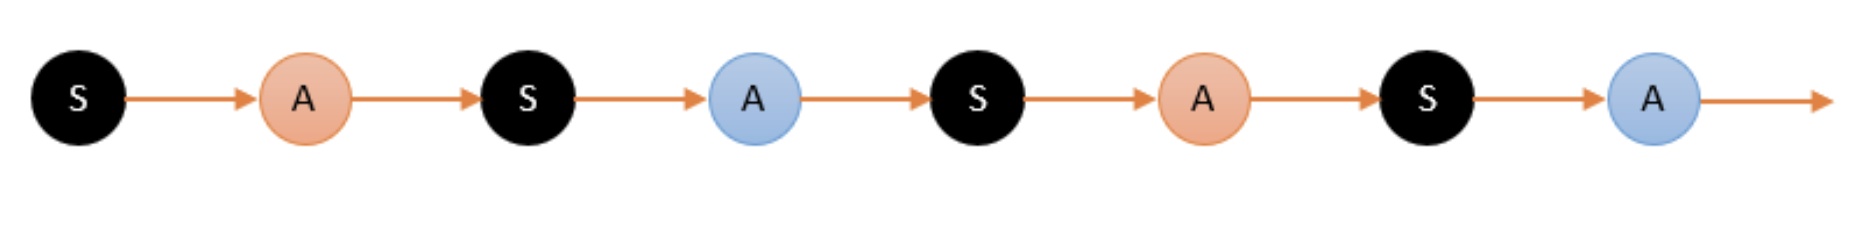
\includegraphics[width=1\textwidth]{fig/ReinforcementLearning/AlphaZero_Decision_Process_States.png}
\end{figure}

图中的S代表状态,A代表动作。红色A和蓝色A分别代表两名玩家的动作。

\begin{itemize}
\setlength{\itemsep}{0pt}
\setlength{\parsep}{0pt}
\setlength{\parskip}{0pt}
    \item 面对S,红方选择动作,让状态改变,进入下一个状态S'。
    \item 面对S',蓝方选择动作,改变状态,再进入一下个状态
\end{itemize}

双方轮流进行动作,(当然,也可以不是轮流,而是由其他规则控制下的执行顺序。)。最终产生图中的一条线路,直到分出胜负,进入最终状态。

我们可以把胜负理解成奖励。但和马可洛夫链不一样,这里的奖励对于双方来说是不一样的,而且是刚好\textbf{相反的}。也就是说,玩家A获得胜利,他的奖励是1。但同时,他的对手就是失败,获得的奖励就是-1。

我们之前也说过,马尔科夫链其实是马尔科夫树。在这里我们也可以画成一棵树的形式,而这条线路,这棵树的一条边。
\begin{figure}[H]
    \centering
    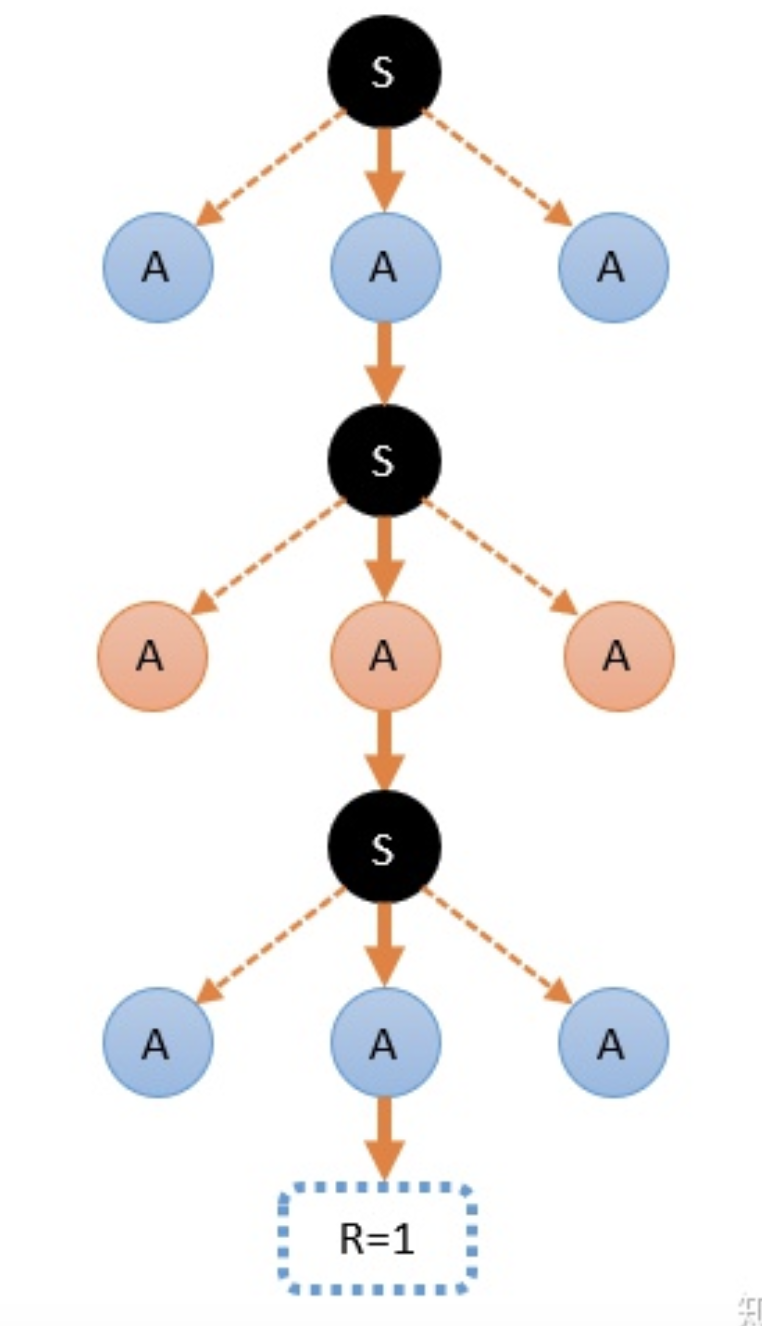
\includegraphics[width=.3\textwidth]{fig/ReinforcementLearning/AlphaZero_Markov_Tree_Example.png}
\end{figure}

在围棋等一些棋类项目,环境是没有不确定性的。所以在这里并没有把状态转移概率画出。而是更关注双方的策略。

由于目标不一样,所以双方的策略目标也是不一样:
\begin{itemize}
\setlength{\itemsep}{0pt}
\setlength{\parsep}{0pt}
\setlength{\parskip}{0pt}
    \item 红方的策略的目标是让红方胜出,获得奖励 +1,的同时,会让蓝方的奖励 -1;
    \item 反之,蓝方的策略是让蓝方胜出,获得奖励 +1,的同时,会让蓝方的奖励 -1。
\end{itemize}

也就是说,\textbf{双方的策略目标都是最大化自己的奖励,同时最小化对手的奖励,这就是最原始的MiniMax思想}。

所谓能接受,就是无论双方自己想着怎样调整策略,也不可能获得更多的奖励了。这个时候,我们就成为双方达到了\textbf{纳什均衡}。

纳什均衡通常并不是最优策略,但可以说是最保险的策略。他是一种防守策略,不让对手占便宜的同时,抓住对手每一丝的破绽。从而不断降低对手的胜率。

但是MiniMax方法有一个很大的限制,就是我必须知道所有可能结果,我们才能通过从下往上的MiniMax获得最优解。在很多时候,这几乎是不可能的:
\begin{itemize}
\setlength{\itemsep}{0pt}
\setlength{\parsep}{0pt}
\setlength{\parskip}{0pt}
    \item 动作空间太大,可选的动作越多,意味着MiniMax树就越宽;
    \item 戏的步数通常比较多,这就意味着这棵树将会很深;
\end{itemize}

以一般的算力,根本没办法计算这么多的节点。

\textbf{蒙地卡罗搜索树(简称:MCTS)}就是希望通过抽样的方式,解决这一问题。

\subsection{蒙地卡罗搜索树}
回顾前面介绍的马尔科夫树,蓝色A表示蓝方动作,红色A表示红方动作。中间实线箭头,表示目前双方按照自己的策略,产生一条线路。最终蓝方获胜,获得奖励+1.
\begin{figure}[H]
    \centering
    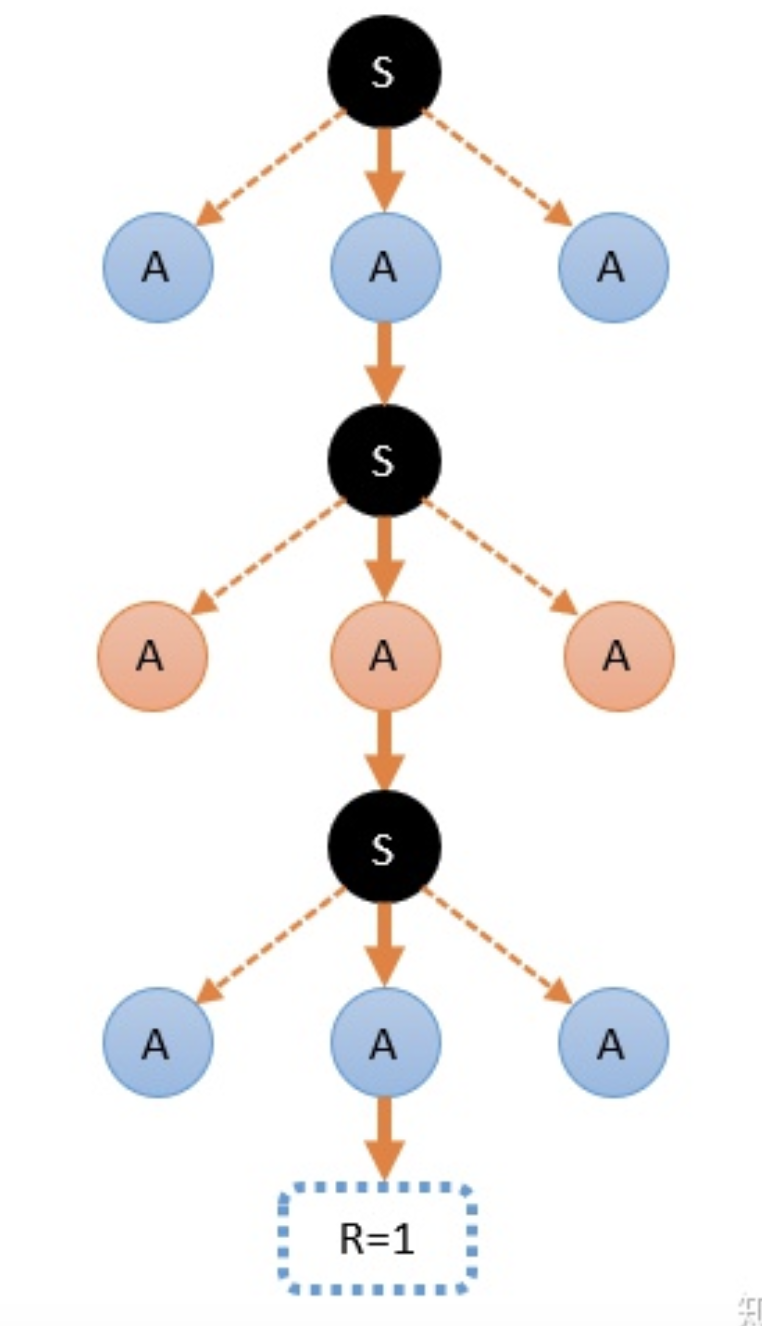
\includegraphics[width=.3\textwidth]{fig/ReinforcementLearning/AlphaZero_Markov_Tree_Example.png}
\end{figure}

蓝方开始迭代自己的策略,思路其实很简单:因为这次赢了,所以当下次我遇到同样的局面(state)的情况下,我会增加我这次行为的概率。

红方的迭代思路也很简单:输了肯定是因为我的选择不好,所以遇到局面(state)的情况下,减少这次行为的概率。调整后,下一次搜寻线路的时候,可能就是别的线路。
\begin{figure}[H]
    \centering
    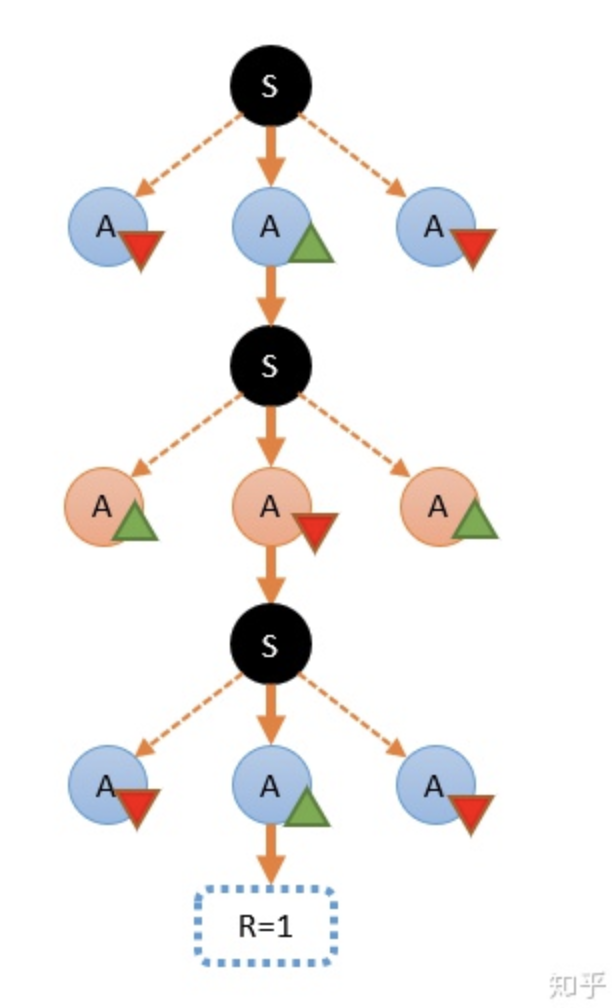
\includegraphics[width=.3\textwidth]{fig/ReinforcementLearning/AlphaZero_Markov_Tree_AB_Selection_Example_1.png}
\end{figure}

大家看:一开始蓝方的选择还是原来中间的A,因为这个动作能给蓝方带来胜利,所以蓝方坚持自己的选择。但红方的选择可能就不一样了。因为上一次中间的动作A带给他失败了,所以它会降低这个动作的选择概率,我们假设红方这一次选择了右边的线路。
\begin{figure}[H]
    \centering
    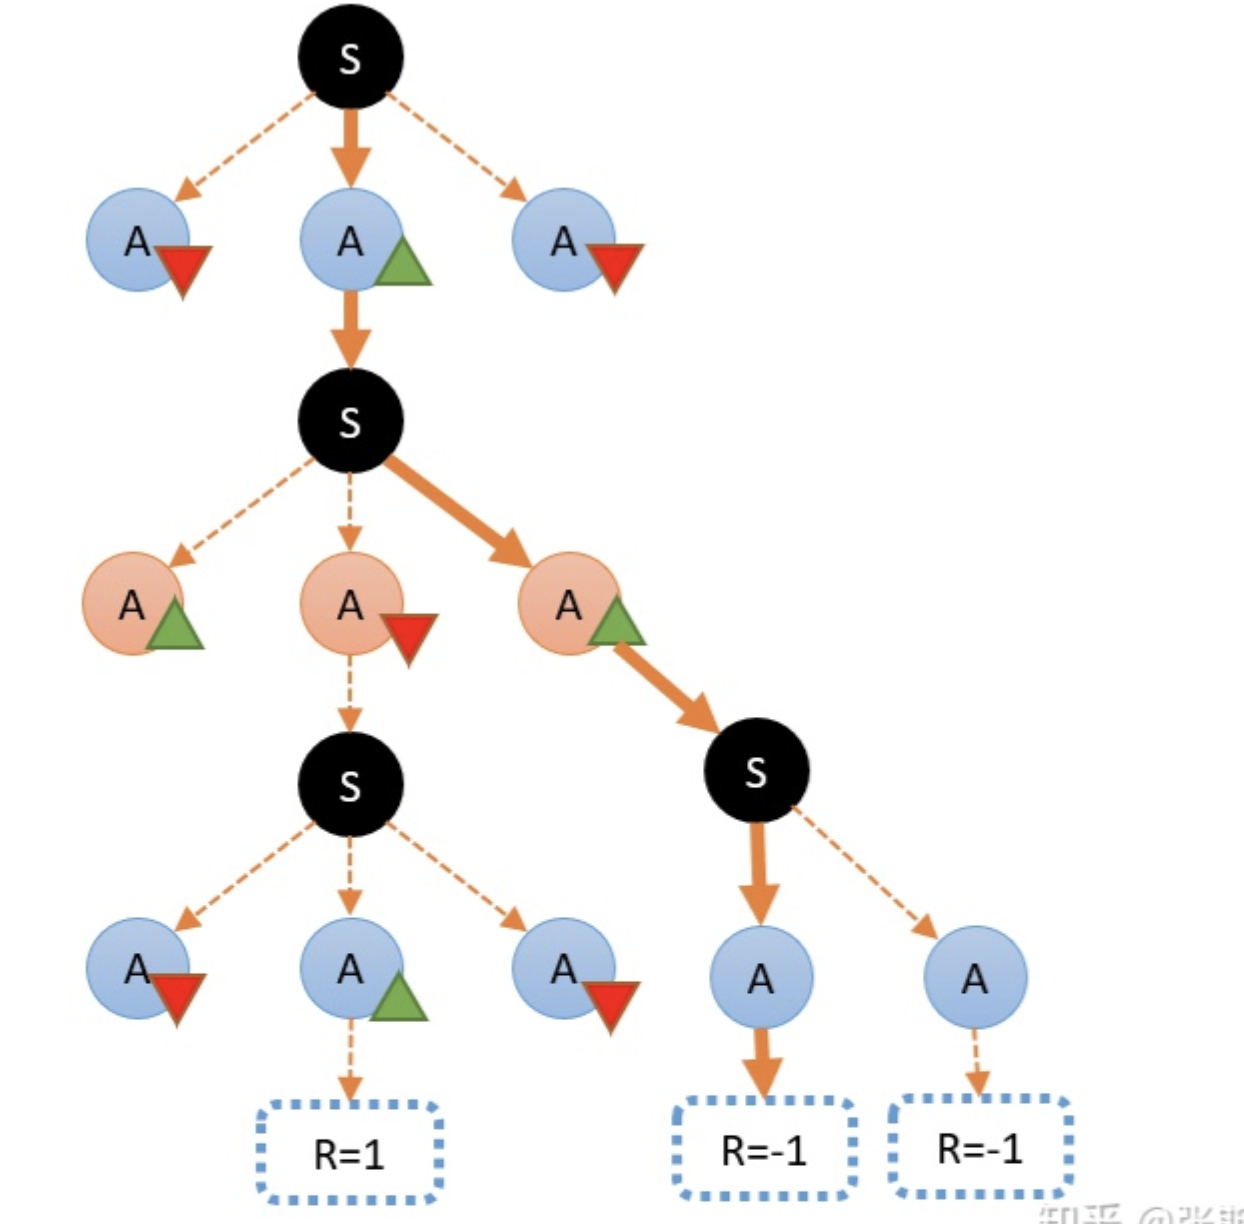
\includegraphics[width=.3\textwidth]{fig/ReinforcementLearning/AlphaZero_Markov_Tree_AB_Selection_Example_2.png}
\end{figure}

最终结果,当然有可能好,也有可能差。但经过多次尝试,就能找出一条接近纳什均衡的线路。这是不是有点像PG算法,按照最后结果,提升自己选择的概率?但这只是一个类比,实际上MCTS远不止如此。MCTS选择动作,并不是按照一个单纯按照动作的概率分布去执行,而是用置信区间上界(UCB)进行。在讲UCB之前,我们先快速了解一下多臂老虎机问题。

\subsection{多臂老虎机问题}
多臂老虎机的问题是这样的。我们假设有这样一排老虎机(假设有4台吧。),每一台老虎机设定的奖励分布都是不一样的。有的10\%的中奖率,有的1\%中奖率,诸如此类。现在我们有1000个硬币,每个硬币允许我们拉动其中一个老虎机一次。并获得奖励。

我们怎样才能获得最多的奖励呢?假设我们已经知道每个老虎机奖励的中奖率,或者老虎机的获得奖励的\textbf{期望}。这个问题就好办了:我们只需要把所有的硬币投到\textbf{期望最大}的老虎机就可以了。但问题是,赌场的老板并不会告诉我们每台老虎机的\textbf{真实期望}。

虽然我们不知道,但我们可以试出来(抽样)。我们可以在一台老虎机投入n个硬币,然后看这个老虎机能吐出多少奖励。最后平均一下,就得到我们要的\textbf{期望奖励了}。这个期望奖励是根据我们抽样后进行的合理猜测。因为这是我们真金白银的经验所得。根据大数定律,我们也有理由相信,当我们投入硬币越多,\textbf{猜测和真实值就越准确}。

我们把希望探索某个老虎机的期望奖励或者中奖率的行为,称为\textbf{探索性}的行为,目的是了解老虎机的属性。另一方面,我们也希望把更多的资源投入到最高中奖率的老虎机,\textbf{开发}中。这个的核心就是许多强化学习要解决的问题——\textbf{探索和开发之间的矛盾}。

\subsection{置信区间上界UCB}
置信区间上界就是其中一种解决方案。UCB这个方法并不常用,在基础的算法中很少用到。目前只有在AlphaZero中用到,并且AlphaZero是用了一种变形的方式。我们在这里只讲直觉。

首先解释一下,什么叫置信区间。置信区间就是我们划定一个范围,我们有一定的信心,我们要找的东西,会在这个区间里。

UCB的方法这就像我们在海里捞鱼。当我们我们没有雷达探测鱼群,我们只能用超级大的网去捞。但我们现在用雷达探测到鱼群,我们可以用小一点的网去捞,也有同样的信心捞到相同数量的鱼。这里的网,就是置信区间。但通常我们的雷达只能探测到一条鱼,所以我们每探测到一条鱼,我们就要调整我们撒网的点,让撒网的点更近一些。

我们来看一下,置信区间是怎样运作的:
\begin{figure}[H]
    \centering
    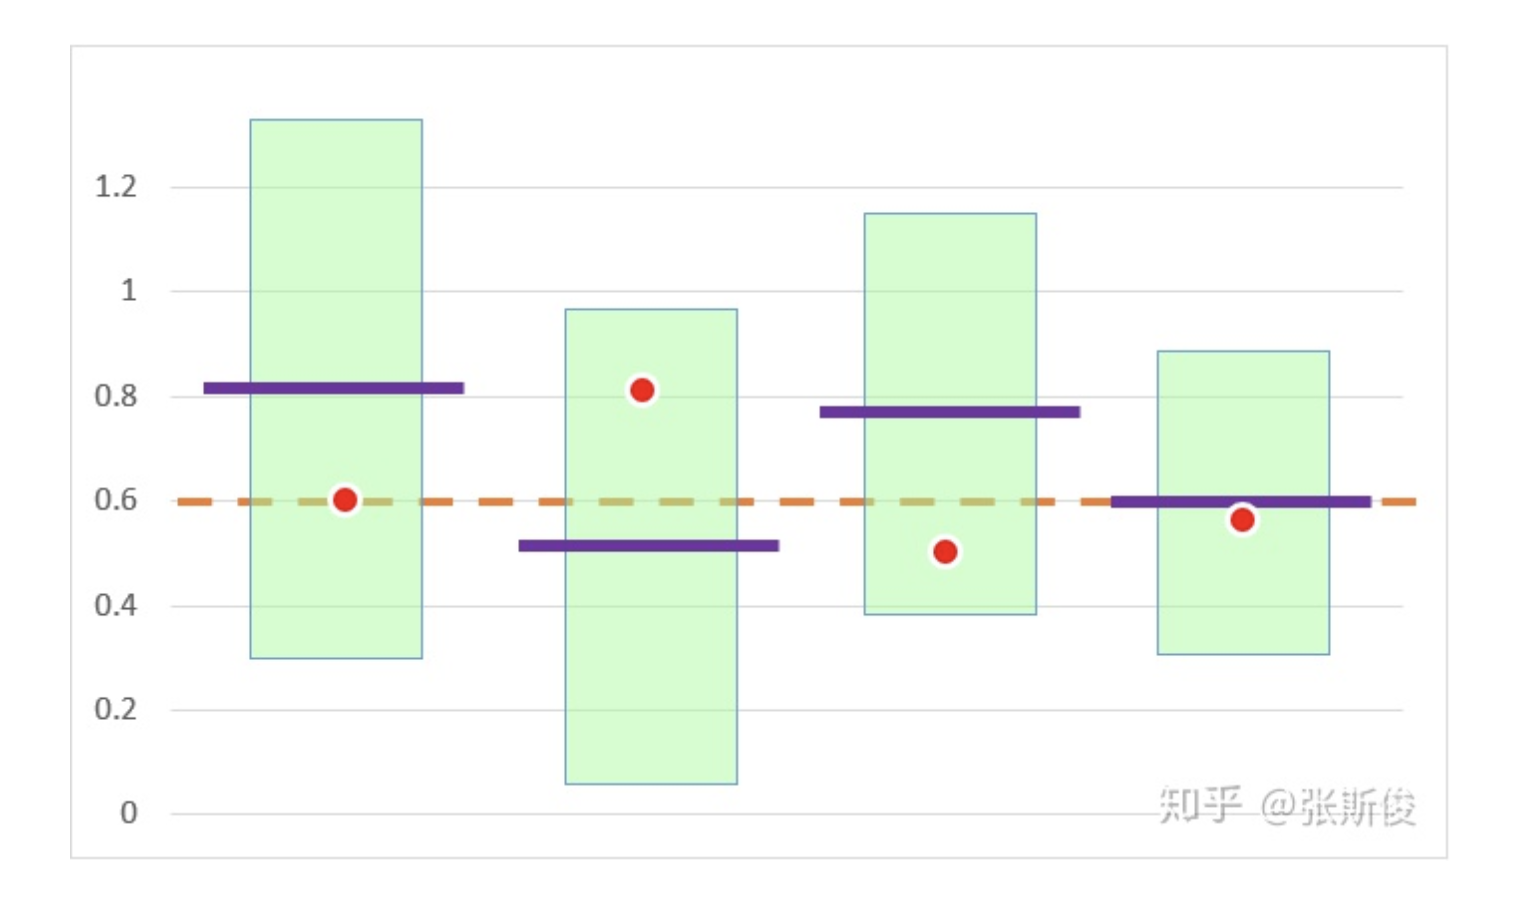
\includegraphics[width=.6\textwidth]{fig/ReinforcementLearning/AlphaZero_UCB_Confidence_Interval_1.png}
\end{figure}
图中,从左到右,分别是4次抽样(红点)和置信区间的变化的示意图。虚线表示真实分布的平均值。所以采样出来的点,都会在虚线的上下附近出现;绿色框代表置信区间,蓝色线代表置信区间的中心。

我们先来给一个区间,认为真实分布的均值很可能会出现在这个区间内。当然,这个区间一开始可以很大。我们希望这个区间的中心能够根据抽样的结果,逐渐地往真实区间靠近。

现在我们从真实分布抽出第一个点。这个点小于我们预估的区间的中心。所以我们让置信区间往下挪动。由于我们比之前多了一个采样点的,所以我们比之前更有理由相信,区间内包含了我们要找的期望值。所以我们把区间压小一点。

第二次抽样,我们得到的点相对于置信区间中点要更大,所以我们把置信区间往上挪动,并把置信区间大小缩小一点。

这样经过多次,我们的置信区间就非常接近我们要的期望值了。

现在我们总结一下置信区间的工作方式:
\begin{itemize}
\setlength{\itemsep}{0pt}
\setlength{\parsep}{0pt}
\setlength{\parskip}{0pt}
    \item 把中间值往抽样的方向挪动。就像探测到了一条鱼的位置,网稍稍往这条鱼挪动一点;
    \item 置信区间缩小。网的大小可以缩小一点,因为我更有信心能够用更小的网捞到鱼了。
\end{itemize}

在多臂老虎机问题中,我们的目标只需要找\textbf{期望最大}的老虎机。所以,并不需要知道所有老虎机的期望。我们只需要找到最大的就可以了。

如图,我们假设有4个老虎机,其真实的期望值如虚线所示。
\begin{figure}[H]
    \centering
    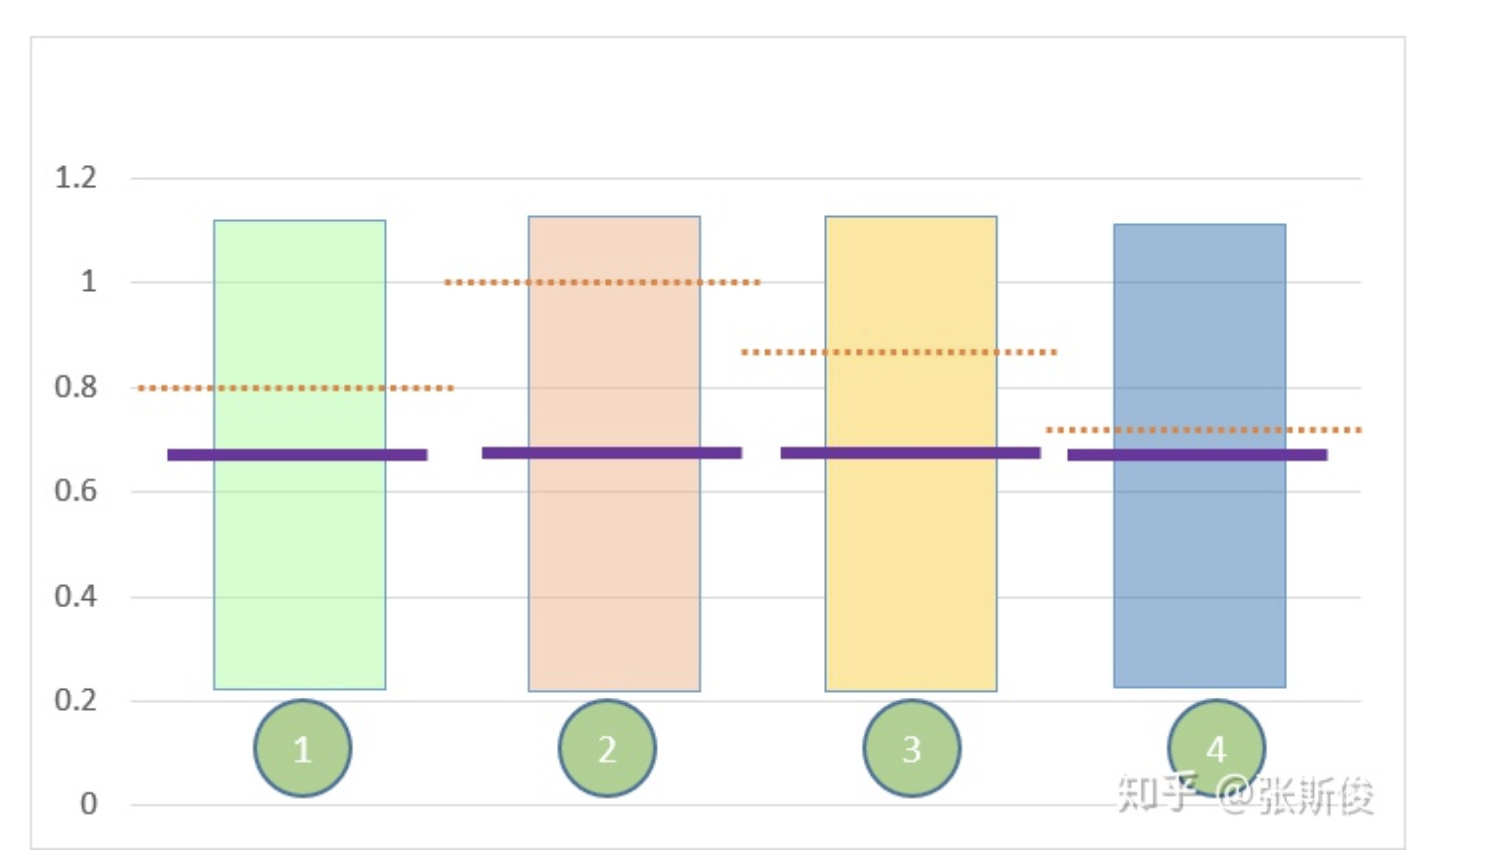
\includegraphics[width=.6\textwidth]{fig/ReinforcementLearning/AlphaZero_UCB_Confidence_Interval_2.png}
\end{figure}

一开始,我们设置一个很大的置信区间。保证这个置信区间能够包含到我们要寻找的期望值。我们从第一个老虎机开始。按顺序进行抽样。经过一轮抽样,移动和缩小置信区间,我们发现置信区间变成这样:
\begin{figure}[H]
    \centering
    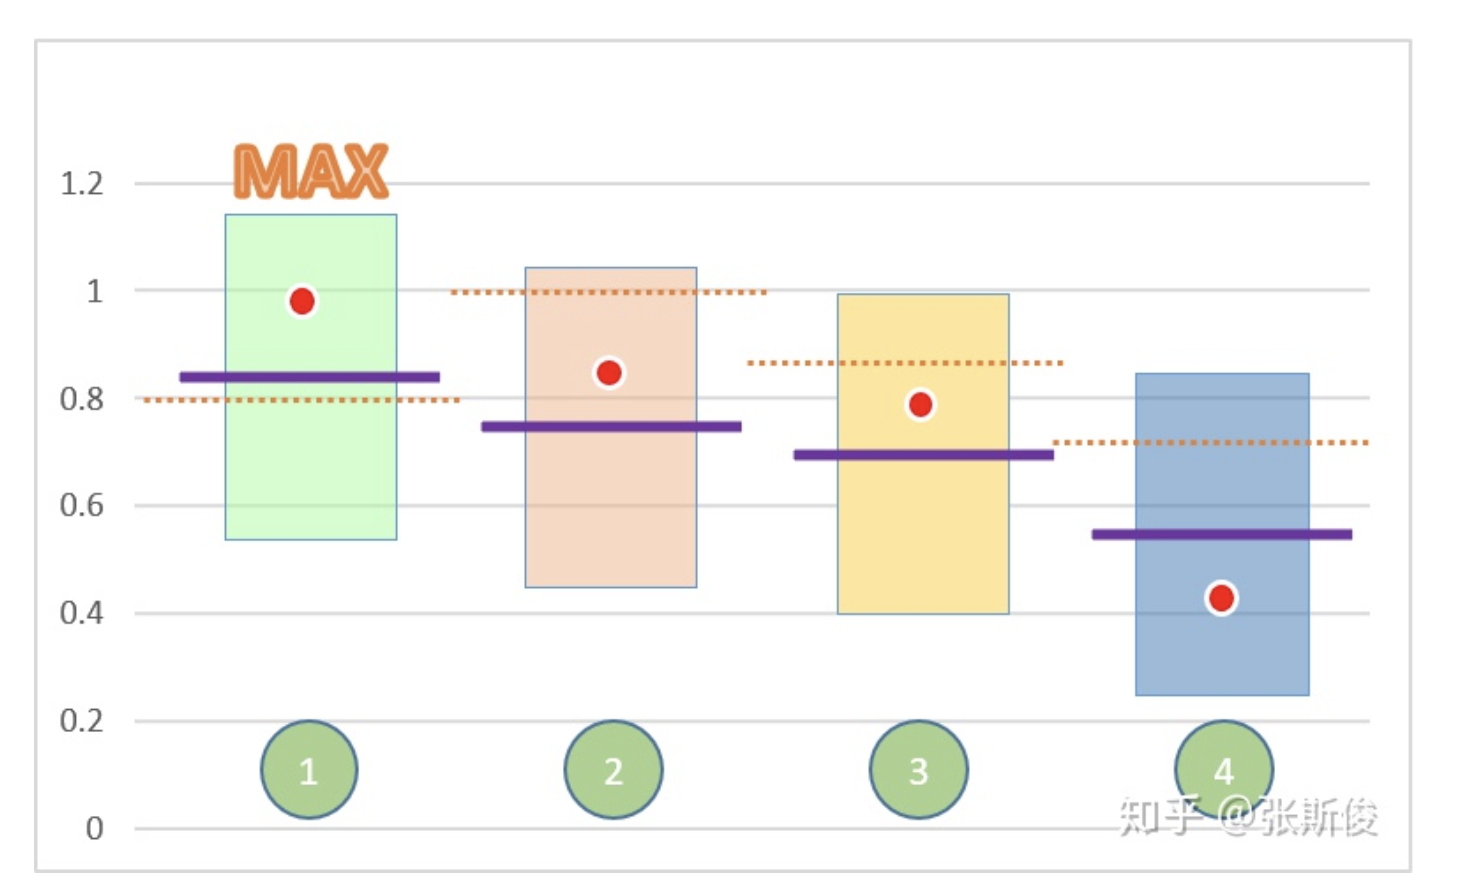
\includegraphics[width=.6\textwidth]{fig/ReinforcementLearning/AlphaZero_UCB_Confidence_Interval_3.png}
\end{figure}

1号老虎机的置信区间的\textbf{上限}是最大的。有同学可能会说,不是应该2号的期望最大吗?是的,但抽样是带有一定的随机性的,好像这一次,1号老虎机的抽样就比2号要大。所以1号会向上挪动更大一点。目前,1号老虎机的置信区间是\textbf{最大上限最高},所以我们选择1号:
\begin{figure}[H]
    \centering
    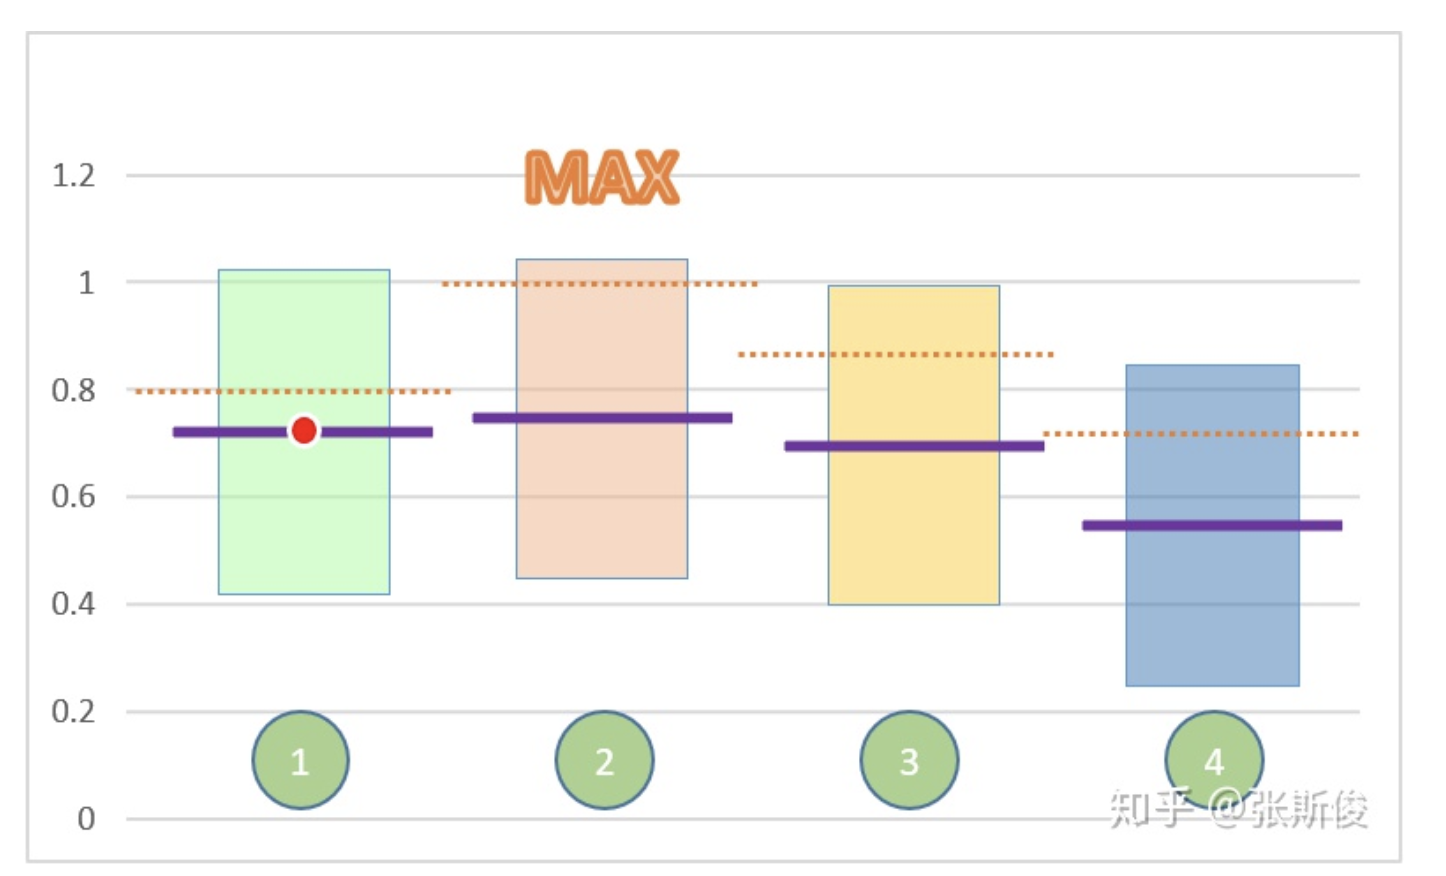
\includegraphics[width=.6\textwidth]{fig/ReinforcementLearning/AlphaZero_UCB_Confidence_Interval_4.png}
\end{figure}

继续抽样后,1号抽样果然回归到他的正常期望,所以1号的置信区间往下挪,并且置信区间缩小。现在2号的置信区间上限是4个老虎机中最高的。所以我们选择2号:
\begin{figure}[H]
    \centering
    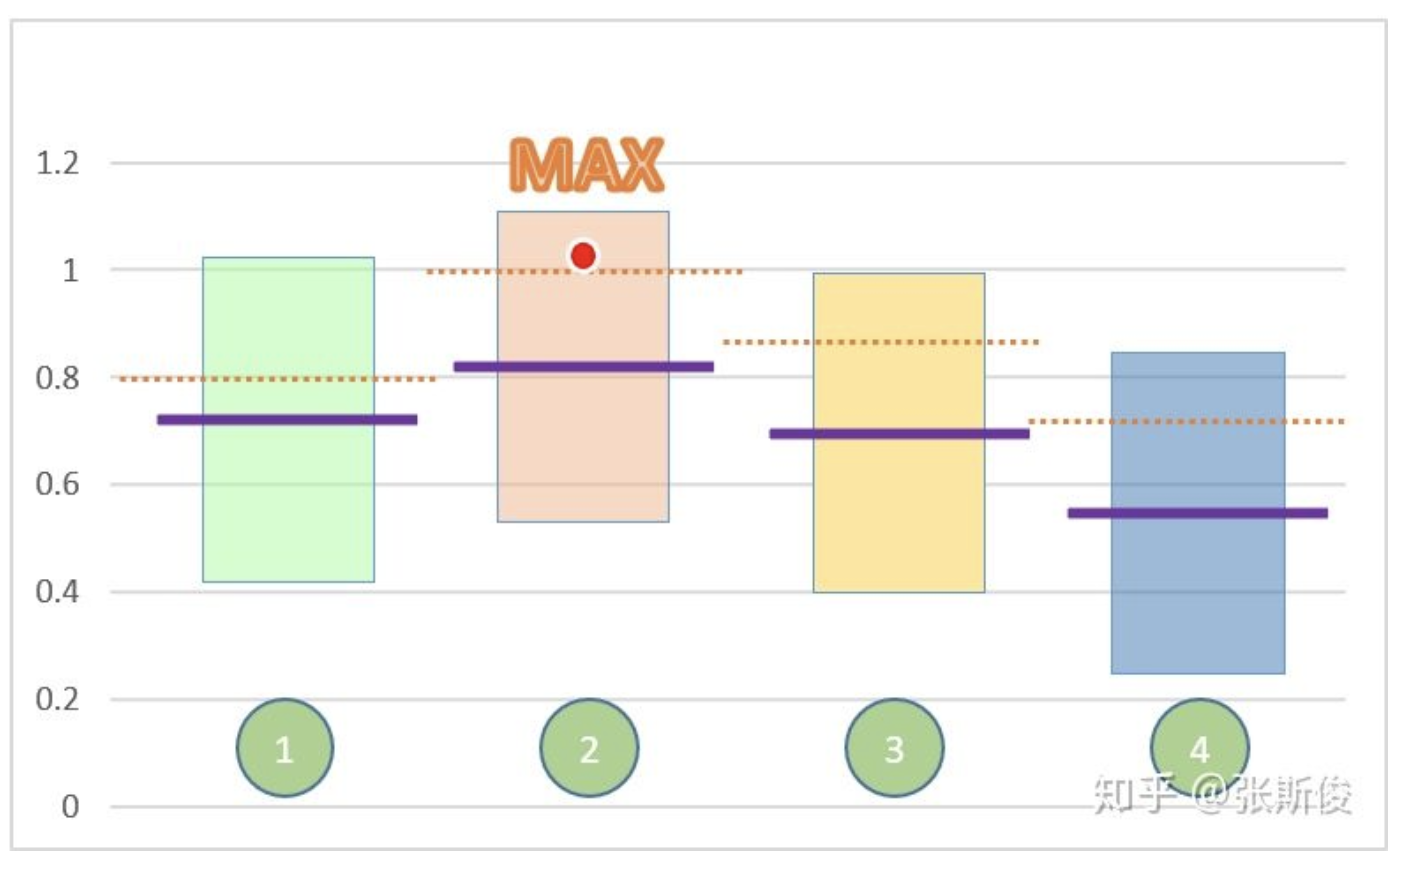
\includegraphics[width=.6\textwidth]{fig/ReinforcementLearning/AlphaZero_UCB_Confidence_Interval_5.png}
\end{figure}

继续抽样后,2号的置信区间上调,并缩小。但仍然是最大的,所以往后多次很可能都会选择2号。直到1号的置信区间上限出现比2号更大。但由于1号的真实期望是比较低的,所以抽样大概率会是的1号的置信区间下调,2号会重夺第一的位置。并一直进行下去。
\begin{figure}[H]
    \centering
    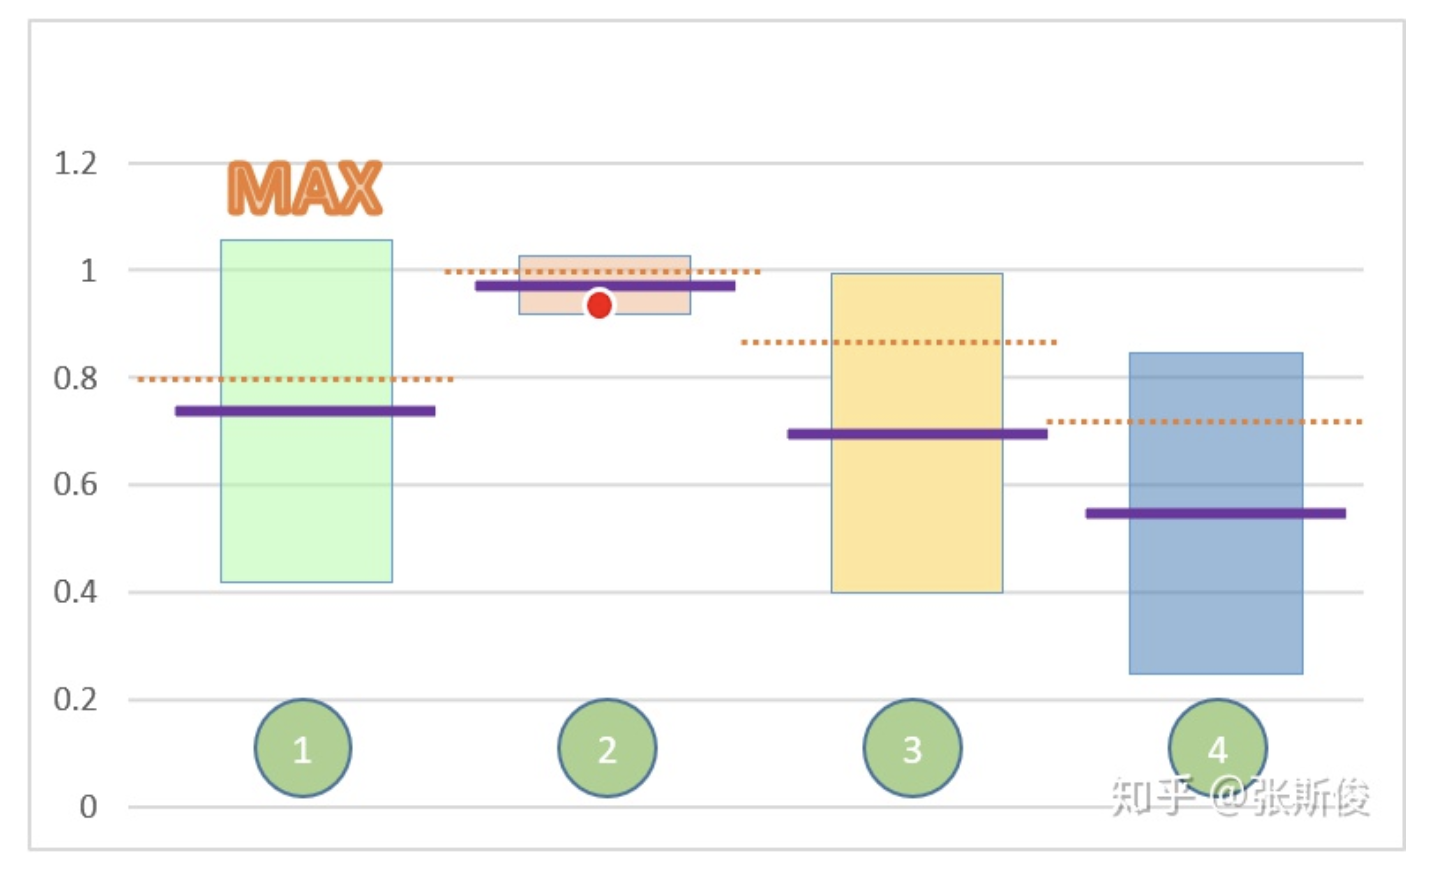
\includegraphics[width=.6\textwidth]{fig/ReinforcementLearning/AlphaZero_UCB_Confidence_Interval_6.png}
\end{figure}

从上面的过程能看到,UCB可以虽然并没有找出所有老虎机的期望,但很快就找出了期望值较高老虎机,让资源能够更多投入到开发中去。

\subsection{重新理解蒙地卡罗搜索树MCTS}
MCTS分为3步,我们逐步来看:
\begin{enumerate}
\setlength{\itemsep}{0pt}
\setlength{\parsep}{0pt}
\setlength{\parskip}{0pt}
    \item select, 选择动作,选择动作就要用到我们刚才说的UCB;
    \item expand, 扩展节点;
    \item update, update就是之前我们讲到的,把胜负的评价返回给每一次的动作;
\end{enumerate}

为了大家能够更加了解这一过程,我们把一些数据结构画出来。我们来做一个过程的演示。
\begin{figure}[H]
    \centering
    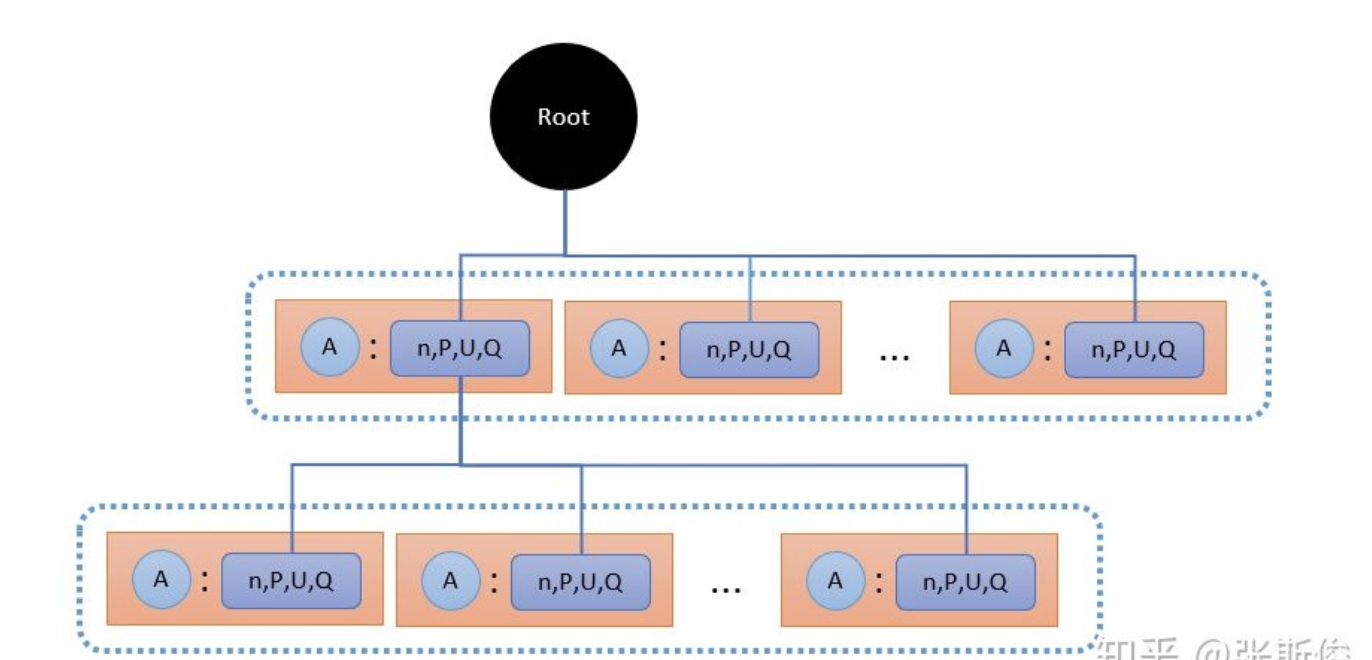
\includegraphics[width=.8\textwidth]{fig/ReinforcementLearning/AlphaZero_MCTS_1.png}
\end{figure}

MCTS中的每个节点,表示一个动作。同时记录以下一些信息。
\begin{itemize}
\setlength{\itemsep}{0pt}
\setlength{\parsep}{0pt}
\setlength{\parskip}{0pt}
    \item n: 表示该节点被访问次数。我们会从根节点出发,进行多次的尝试。每次尝试会经过的节点,n将会加1
    \item P:动作对应的概率,可以理解为策略。
    \item U:记录UCB上限
    \item Q: 该节点价值
\end{itemize}

需要说明的是,根节点其实也是一个包含n,P,U,Q信息的节点,不过我们并不关心根节点,因为我们想知道的是,我们应该选哪个动作。

现在我们开始流程:

(1). \textbf{Select(选择)}:从根节点,选择1个动作执行,直到叶子节点。如图,这次执行路径由红色线条表示。
\begin{figure}[H]
    \centering
    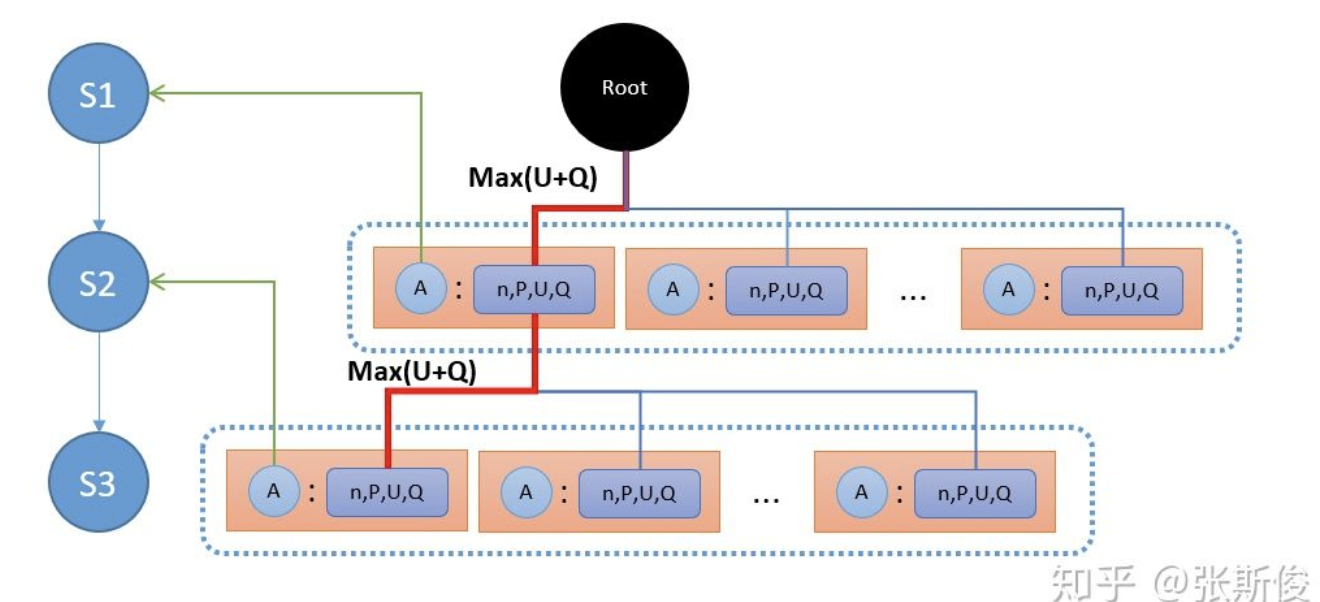
\includegraphics[width=.8\textwidth]{fig/ReinforcementLearning/AlphaZero_MCTS_2.png}
\end{figure}

那动作选择的理由是什么呢?就是UCB。不过AlphaZero在UCB的基础上做出了修改。我们直接给出alphazero中用的UCB计算公式:Max(Q+U),其中U的公式:
$$
U = c_{puct}P\frac{\sqrt{\sum N'}}{1+N}
$$

我们选择最大的U+Q值的动作,然后执行。状态将会随之变化,进入新状态。

(2). \textbf{Expand(扩展)}:到了叶子节点,如果还没到最终状态,我们开始扩展。我们需要先确定,我们当前能够执行的动作有哪些。

\textbf{用神经网络进行预估,需要预估两个值}:
\begin{itemize}
\setlength{\itemsep}{0pt}
\setlength{\parsep}{0pt}
\setlength{\parskip}{0pt}
    \item 当前叶子节点的 价值(leaf\_value) Q;
    \item 从这个叶子节点扩展出去的新叶子,他们的P值;
\end{itemize}

把这些动作都对应到一个MCTS节点。在实做上,我们会用字典结构进行对应。
\begin{figure}[H]
    \centering
    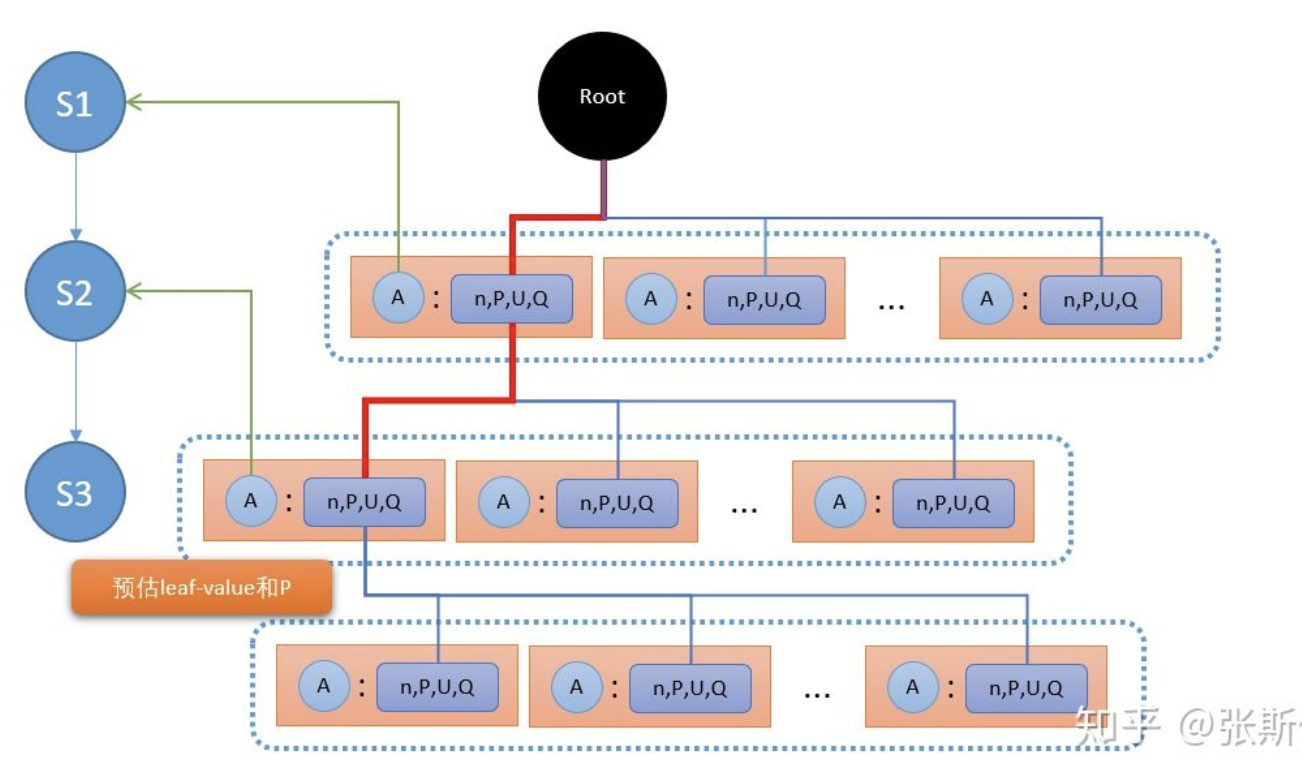
\includegraphics[width=.8\textwidth]{fig/ReinforcementLearning/AlphaZero_MCTS_3.png}
\end{figure}

如图,在扩展后,这棵树将会多一层。

(3). \textbf{update(更新)}:在更新的时候,我们会回溯更新,也就是从当前叶子节点,一直回到根节点。
\begin{figure}[H]
    \centering
    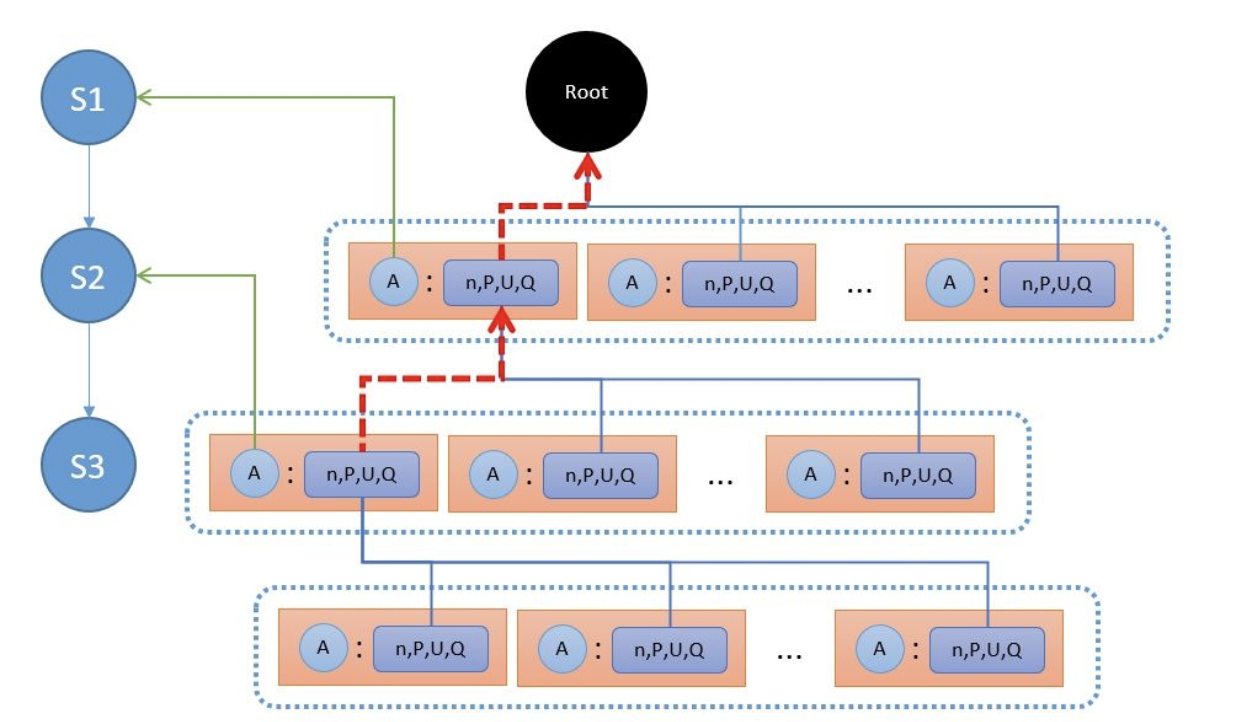
\includegraphics[width=.8\textwidth]{fig/ReinforcementLearning/AlphaZero_MCTS_4.png}
\end{figure}

更新的内容包括两个:
\begin{itemize}
\setlength{\itemsep}{0pt}
\setlength{\parsep}{0pt}
\setlength{\parskip}{0pt}
    \item 沿途经过的节点路径,次数加1;
    \item 我们在expand的时候,用神经网络预估了叶子节点A的价值(leaf\_value),用来更新沿途节点的Q值。更新方式用增量更新即可,因为我们已经会记录经过的次数了;
\end{itemize}

这里需要更详细说明一下原理:
\begin{figure}[H]
    \centering
    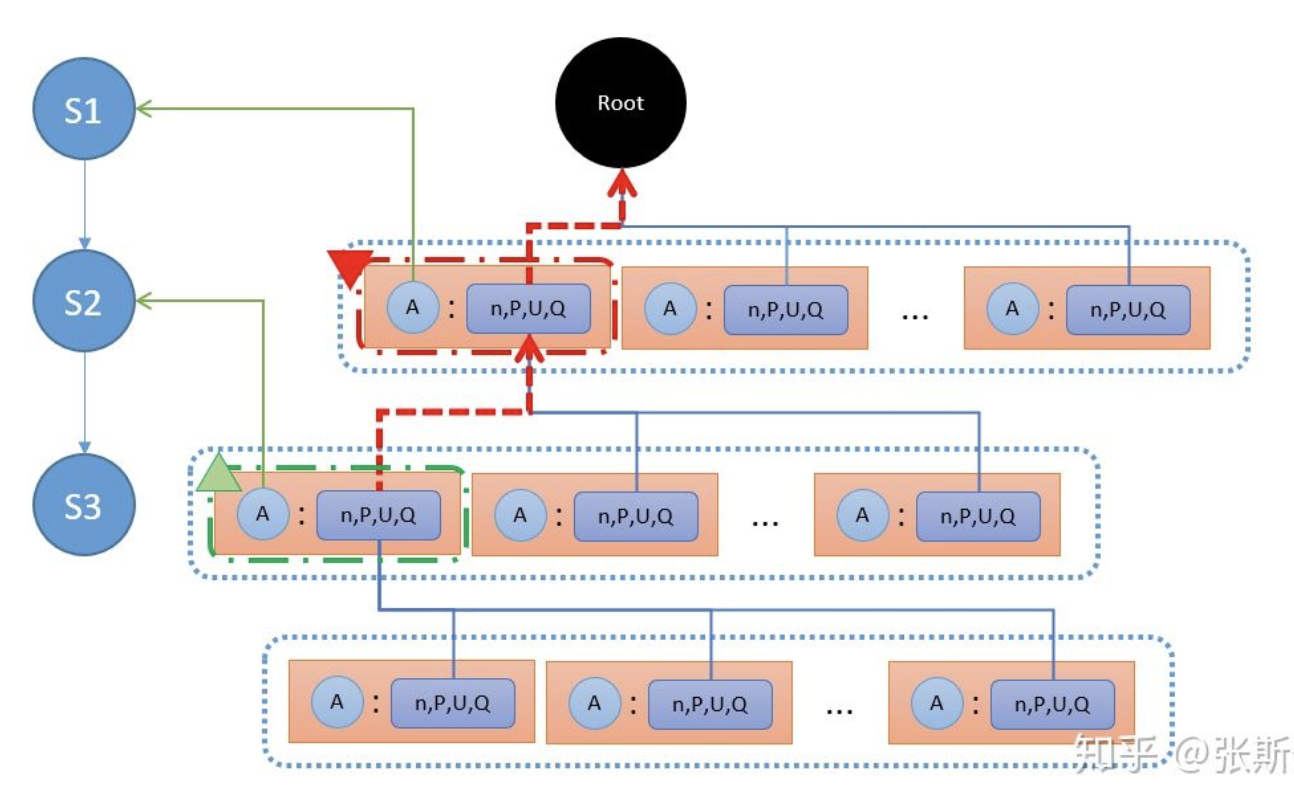
\includegraphics[width=.8\textwidth]{fig/ReinforcementLearning/AlphaZero_MCTS_5.png}
\end{figure}

我们假设叶子节点A,表示玩家甲,面对状态 S2 的动作(图中绿框部分)。并预估了叶子价值。叶子价值越大,表示这个动作对甲越有利,甲也越应该选择A动作。

这个动作对甲越有利,对手乙就应该降低达到S2局面的概率,也就是说,应该减少上手的动作的价值(图中绿框部分)。

所以,我们要针对不同的双方的动作的执行顺序进行更新。叶子节点的玩家的所有动作,都应该正向更新leaf\_value。他的对手应该反向更新leaf\_value。

我们下一次进行select,会同样会以 Max(Q+U) 作为选择的依据。现在我们对Q进行修改。下一次select就可能会执行其他路径。当执行次数足够多,就会达到一个平衡状态——你没能占我的便宜,我也没能占你的便宜。我们说这样就达到了一个纳什均衡。

\textcolor{red}{最终,我们会选择经过次数最多的那个动作作为我们真正选择的标准。注意:这里不是Max(Q+U)。也就是说,我们最终选择,是基于纳什均衡的选择}。

\begin{framed}
\textbf{相关公式的理解}

我们说完MCTS的流程,现在回来再看一下这关键的公式,我们先看这部分:
\begin{figure}[H]
    \centering
    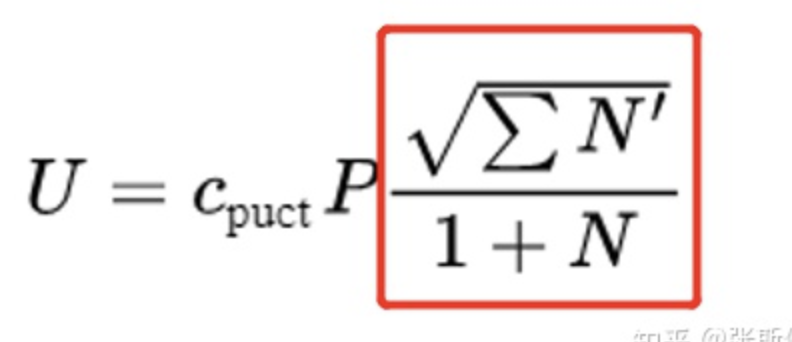
\includegraphics[width=.2\textwidth]{fig/ReinforcementLearning/AlphaZero_MCTS_Eq_1.png}
\end{figure}

公式中,$N'$表示父节点被访问次数,$N$表示当前节点被访问次数。这部分就充满了UCB的思想了。为了方便讨论,我们先给这部分起个名字\textbf{UCB系数}。

我们举个例子,某父节点下有两个子节点A1和A2,被访问次数分别是$N1$和$N2$。由树结构我们知道,如果我们访问过一个节点,那么我们肯定也访问过他的父节点。所以我们可以知道$N1 + N2 = N'$:
\begin{figure}[H]
    \centering
    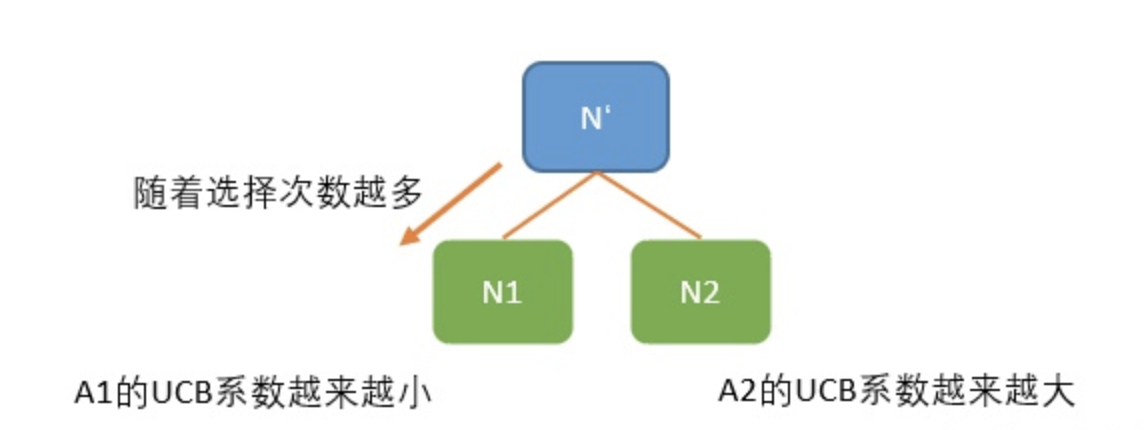
\includegraphics[width=.8\textwidth]{fig/ReinforcementLearning/AlphaZero_MCTS_Eq_2.png}
\end{figure}

当某个子节点被访问次数越来愈多,例如,$N1$越来越大,父节点被访问次数和$N1$的差距将会越来越小,UCB系数也会越来越小。但相应的,它的兄弟节点是不变的,但父节点被访问次数多了。所以他们的UCB系数将会越来越大。

一边系数是越来越小,但兄弟节点的系数将会越来愈大。当访问次数足够多的时候,也会尝试进行\textbf{探索性}行为。这就是这个公式中UCB的意义。
\end{framed}

\begin{framed}
\textbf{P 和 Q 的理解}

我们之前说过,P可以理解为策略,Q可以理解为行为的价值。当我们忽略UCB系数的时候,我们需要 \textbf{Max(Q+U)},相当于 \textbf{Max ( Q + C * P )}, 其中C是一个超参数。

于是从这个公式我们可以这样理解(当然这只是我个人理解):
通过我们之前对强化学习的理解,Q和策略通常是一致的。因为越有价值的动作,证明它未来获得的奖励越多,所以我们的策略需要更倾向使用这个动作。

AlphaZero可能觉得,如果让学习策略同时学习动作的Q值,学习将更有效率。所以AlphaZero的网络是一个双引擎学习网络。

这样我们就可以理解\textbf{参数C,是策略和动作Q价值的换算单位}。它把Q值和策略联系了起来,我们可以把它称为\textbf{效用}。

现在我们可以开始理解AlphaZero的网络了。
\begin{figure}[H]
    \centering
    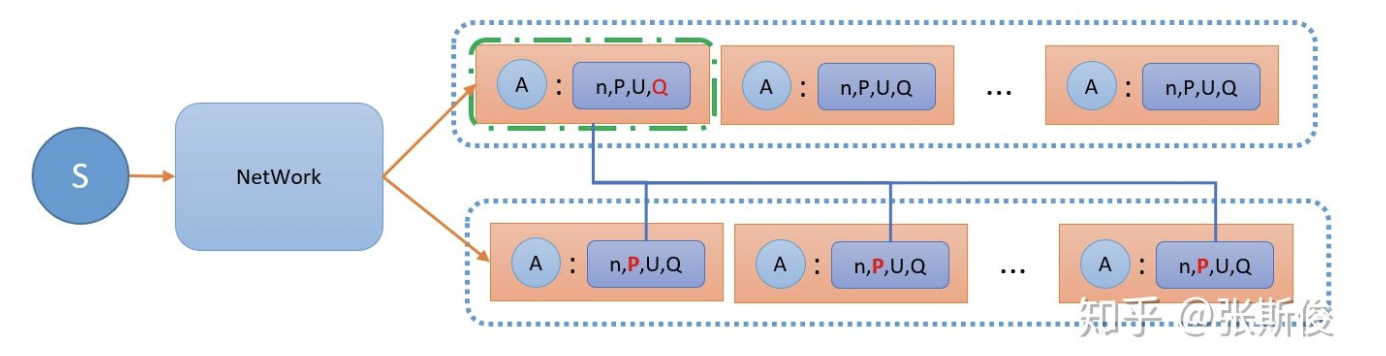
\includegraphics[width=.8\textwidth]{fig/ReinforcementLearning/AlphaZero_MCTS_Eq_3.png}
\end{figure}

正如我们之前说的\textbf{AlphaZero的网络是一个双引擎学习网络。它既要学动作价值Q,也要学策略 P}。

所以网络会吃入一个状态,\textbf{输出Q值,也输出叶子节点的所有动作的策略P值}。

注意:网络只用在MCTS扩展叶子节点(expand)之前。一旦expand出来之后,就没网络什么事了。

这里可能要多说一句,有的同学可能不明白,为什么AlphaZero需要网络呢?就MCTS不好吗?按上面说的,纯MCTS就能达到纳什均衡的效果呀。是的,其实AlphaZero的核心真不是网络,是MCTS。网络的作用是辅助MCTS。

或者说,用网络去\textbf{保存}(或者\textbf{拟合})MCTS中,每个动作节点的Q和P。这就有点像我们在学DQN的时候,就是用网络去保存Qtable里面的Q值一样。只不过在AlphaZero里,我们的神经网络不是去保存一个表格,而是保存一棵树而已。

纯MCTS在开始使用的时候,会使用平均策略和相等的Q值代替网络的估值。当经过一段时间后(如果MCTS树不是很大的话),纯MCTS的确也能够达到纳什均衡状态。但当我们有一个网络去保存之前学到的Q和P作为叶子初始化,MCTS自然更快地学习到嘛。

所以,当我们在玩一种比较简单的游戏,例如井字棋,这种状态空间较少的游戏,MCTS也能很快达到均衡状态,网络感觉上是没什么用的。但在围棋这种状态树特别深特别宽的棋类,网络的优势就体现出来了。

我在实战中用过AlphaZero算法玩一种类似21点的游戏,并尝试用纯MCTS和AlphaZero进行对战。 在同样模拟步数的情况下,当MCTS运算步数足够多能够探索到树的所有空间时候,AlphaZero和MCTS的胜率相当。但当步数比较少,AlphaZero的优势就很明显了。

说回网络,根据我们之前学到的知识,我们知道网络的学习要设定好目标。AlphaZero是双引擎的网络,就需要两种目标:
\begin{itemize}
\setlength{\itemsep}{0pt}
\setlength{\parsep}{0pt}
\setlength{\parskip}{0pt}
    \item Q的目标:动作价值的目标很简单。因为最终胜利和失败会产生结果z,也就是对胜利和失败者的reward。我们让Q向z更新。
    \item P的目标:P的目标不是去靠近MCTS节点中的P值,因为P值在回溯的时候是不会变化的。但我们之前讲过,MCTS某条路径被访问次数越多,越接近纳什均衡的策略,越应该被我们采用。所以我们策略的目标是把输出的策略向最多访问次数的动作靠近。
\end{itemize}
\end{framed}

\subsection{AlphaZero 总结}
AlphaZero牵涉到的知识点比较多,但最终还是以MCTS作为核心,网络辅助。

(1). MCTS的直觉:我们说MCTS的任务就是找纳什均衡。找的方式是不断进行游戏,然后根据输赢反馈这一路上的动作是否合适。胜利一方提高所有的行为的效用,而失败方减少动作效用。最终就能达到一种均衡的状态。

(2). MCTS的建立:
\begin{itemize}
\setlength{\itemsep}{0pt}
\setlength{\parsep}{0pt}
\setlength{\parskip}{0pt}
    \item select 以Max(Q+U)作为依据选择动作,直到叶子节点;
    \item expand 把叶子节点扩展;
    \item update 把一路上的节点访问次数+1 更新节点的Q值;
\end{itemize}

(3). AlphaZero用的UCB公式,红色部分就是UCB的意味,大家可以对照原来置信区间上界来细品
\begin{figure}[H]
    \centering
    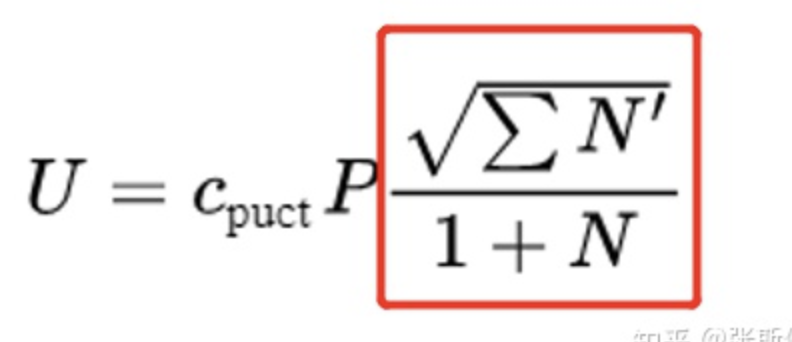
\includegraphics[width=.4\textwidth]{fig/ReinforcementLearning/AlphaZero_MCTS_Eq_1.png}
\end{figure}

当AlphaZero select的时候,我们会用Max(U+Q)。我们可以把U+Q 看成 Q + C * P。其中Q是动作价值,P是策略,C是一个参数,起到一个接通动作和策略之间的桥梁纽带作用。

(4). AlphaZero的网络是一个双引擎网络,既学习价值Q,也学习策略P。Q的更新目标很简单,因为MCTS最终会不断调整。所以我们只需要把输出的Q向经过MCTS修改后的Q靠近即可。MCTS到达平衡状态后,某个选择将会特别多,所以我们把策略向这个动作靠近即可。

总结来说,AlphaZero的思路并不复杂,用一句话来说,就是用深度神经网络辅助MCTS找到均衡点。但其中的细节特别多。

\section{AlphaZero实战}
我们知道MCTS是树的结构,那我们怎样来实现这样一棵树呢?我们先来看叶子结点(TreeNode类)。

\subsection{TreeNode类}
\subsubsection{基本结构}
\begin{python}
def __init__(self, parent, prior_p):
    # 节点结构部分:
    self._parent = parent 	#父节点
    self._children = {}		#子节点,其实是一个字典:字典的key是可用动作;字典的item是子节点。item包括n、Q、u、P等信息
    # 节点属性部分:
    self._n_visits = 0		#该节点被访问的次数   
    self._Q = 0			#这个节点的价值      
    self._u = 0			# 用于计算UCB上限
    self._P = prior_p		# 动作对应的概率
\end{python}

现在,节点我们已经做好了,我们通过select - expand - update三步,慢慢建立起MCTS。

\subsubsection{select}
我们之前说过,select任务,就是按照MAX(Q+U)选择动作,直到叶子节点。我们可以专门写一个函数,计算该节点的 MAX(Q+U),然后用一个Lambda函数,获取能获得MAX(Q+U)对应的动作:
\begin{python}
def get_value(self, c_puct):
    self._u = (c_puct * self._P *
                np.sqrt(self._parent._n_visits) / (1 + self._n_visits))
    return self._Q + self._u
    
def select(self, c_puct):
    return max(self._children.items(), key=lambda act_node: act_node[1].get_value(c_puct))
\end{python}

\subsubsection{expand}
当搜索到叶子节点,但还没到最终状态,我们需要把MCTS继续扩展。
\begin{python}
def expand(self, action_priors):
    for action, prob in action_priors:
        if action not in self._children:
            self._children[action] = TreeNode(parent=self, prior_p = prob)
\end{python}
这就相当于在新的状态下,对各个可能动作估算P,然后把这些动作节点接到父节点。

\subsubsection{update}
我们需要注意,update是每次到达叶子节点,无论是扩展还是已经达到最终状态,都要进行从下到上的更新。

更新的内容包括两项:
\begin{itemize}
\setlength{\itemsep}{0pt}
\setlength{\parsep}{0pt}
\setlength{\parskip}{0pt}
    \item \_n\_visits:途径的节点访问次数+1;
    \item \_Q: 把叶子节点的价值,平均到途径节点的Q中;
\end{itemize}

\begin{python}
def update(self, leaf_value):
    self._n_visits += 1             #更新访问次数

    # 计算leaf_value和之前的Q值的均值
    self._Q += 1.0*(leaf_value - self._Q) / self._n_visits
\end{python}

但需要注意,leaf\_value的更新对当前玩家是正向,而对方是负向的。

所以如果规则类似象棋、围棋,双方轮流下棋,那么我们可以这样实现:我们先按父节点一直往上,但途径都会留下负号。当我们正式更新的时候,就会按照 + - + - 的顺序更新。
\begin{python}
def update_recursive(self, leaf_value):
    if self._parent:
        self._parent.update_recursive(-leaf_value)  #注意这里的符号
    self.update(leaf_value)
\end{python}
\begin{framed}
理解:感觉是应该先更新当前节点的 leaf\_value,再递归向上更新父节点?
\begin{python}
def update_recursive(self, leaf_value):
    self.update(leaf_value)
    if self._parent:
        self._parent.update_recursive(-leaf_value)  #注意这里的符号
\end{python}
\end{framed}

但如果游戏规则不是轮流的,而是按照某个规则有先后手规则。那么我们可以记录出手的顺序,在更新的时候按照这个顺序给正负号。

\subsection{MCTS流程}
现在,我们把整个MCTS树的建立流程整理一下:
\begin{enumerate}
\setlength{\itemsep}{0pt}
\setlength{\parsep}{0pt}
\setlength{\parskip}{0pt}
    \item 首先我们通过select,直到树的叶子节点。注意:我们一边select一边会对执行动作,改变state;
    \item 到达叶子后,我们先看一下是否已经分出胜负了,如果还没有,就进行expand。expand所需的数据,把当前的state放入神经网络,就可以获得;
    \item 如果达到最终状态。那么整理一下奖励;
    \item 反向更新途径节点Q值和访问次数n
\end{enumerate}

\begin{python}
def _playout(self, state):
    node = self._root

    #===select====
    #一直执行select,直到达到叶子节点
    while(1):
        action, node = node.select(self._c_puct)
        state.do_move(action)   
        if node.is_leaf():
            break

    #===Evaluate===
    # 用网络估算动作和对应的策略P,还有节点的Q值
    action_probs, leaf_value = self._policy(state)

    #===expand=====
    #如果还没分胜负,进行expand
    end, winner = state.game_end()
    if not end:
        node.expand(action_probs)

    #如果结束了。
    #如果平局,就设置成leaf_value = 0
    #否则: 如果胜利者是当前的,那么leaf_value = 1, 否则leaf_value = -1
    else:
        # for end state,return the "true" leaf_value
        if winner == -1:  # tie
            leaf_value = 0.0
        else:
            leaf_value = (
                1.0 if winner == state.get_current_player() else -1.0
            )
            
    # update 
    # 向上更新祖先节点。
    node.update_recursive(-leaf_value)
\end{python}

\subsection{Alpha网络}
AlphaZero对网络有一番设计,但通常我们要试验的游戏其实没有围棋那么困难,状态空间要小很多。所以我们的网络也可以稍微简化。我们只需要记着我们需要预估两个值:该节点的Q值和子节点的P值。

经过我们之前的专栏,要做到应该不难的。但我们要关注状态的表达。

\subsubsection{状态表达}
AlphaZero用了17层和棋盘大小一样的矩阵,来表示当前状态。其中:
\begin{itemize}
\setlength{\itemsep}{0pt}
\setlength{\parsep}{0pt}
\setlength{\parskip}{0pt}
    \item 8层矩阵表示\textbf{玩家A}的当前棋子(黑棋)位置和之前7步的棋子位置;
    \item 8层矩阵表示\textbf{玩家B}的当前棋子(白棋)位置和之前7步的棋子位置;
    \item 最后一层,用全0 或者 全1 表示当前执行的玩家是A还是B
\end{itemize}

为什么要这样呢?我想是基于两点原因:
\begin{itemize}
\setlength{\itemsep}{0pt}
\setlength{\parsep}{0pt}
\setlength{\parskip}{0pt}
    \item 如果我们只用当前盘面来表示,比较难以了解当前是谁在下。因为同一个盘面,不同玩家在下,结果明显是不同的;
    \item 把最近8步棋子加入到state,能够帮助机器学习。我们下棋的时候,最重要的固然是当前棋子的位置,但如果我们能记住对方的操作过程,这部分有助于我们研究对方的思路,这相当于多了信息去参考了;
\end{itemize}

当然,这只是AlphaZero的做法。我们在面对实际游戏,可以有不同的处理,但我们可以有这样几个角度:
\begin{itemize}
\setlength{\itemsep}{0pt}
\setlength{\parsep}{0pt}
\setlength{\parskip}{0pt}
    \item 怎样表示当前棋盘或者当前的状态?
    \item 现在是谁在执行,怎样表达?
    \item 之前的状态怎样表示,是否需要表示?
\end{itemize}

\subsubsection{更新目标}
我们来看一下,Q值和P值的更新目标:
\begin{itemize}
\setlength{\itemsep}{0pt}
\setlength{\parsep}{0pt}
\setlength{\parskip}{0pt}
    \item Q的目标:动作价值的目标很简单。因为最终胜利和失败会产生结果winner\_batch,也就是对胜利和失败者的reward。我们让Q向z更新;
    \item P值不会随着MCTS更新,但我们最终的选择的动作,是被访问得最多的动作。这个动作会比较接近均衡策略。所以我们用这个动作来更新P值。所以这里和PG算法的更新是很相似的;
    \item 加入了L2正则化,防止过度拟合。
\end{itemize}

\begin{python}
def train_step(self, state_batch, mcts_probs, winner_batch, lr):
    with tf.GradientTape() as tape:           
        act_probs, value , log_act_probs= self.policy_value

        # value_loss 用 mse 就可以了
        self.value_loss = tf.losses.mean_squared_error(winner_batch,value)

        self.policy_loss = tf.negative(tf.reduce_mean(tf.reduce_sum(tf.multiply(mcts_probs, log_act_probs), 1)))

        #L2权重正则化,防止过拟合
        l2_penalty_beta = 1e-4
        vars = self.model.trainable_weights
        l2_penalty = l2_penalty_beta * tf.add_n([tf.nn.l2_loss(v) for v in vars if 'bias' not in v.name.lower()])

        self.loss = self.value_loss + self.policy_loss + l2_penalty

    #自动求导,常规动作
    grads = tape.gradient(self.loss,self.model.trainable_weights)
    self.opt.apply_gradients(zip(grads,self.model.trainable_weights))
    return loss,value_loss,policy_loss,l2_penalty
\end{python}

\subsubsection{运行框架说明}
虽然AlphaZero的核心是MCTS,但我们要明确:MCTS是会随着游戏进行建立的,但我们要做的是训练好一个网络,能够预测MCTS中节点的Q和P值。

另外,在训练中,其实是不需要对手的。通过MCTS的学习我们知道,MCTS其实可以让玩家自己左右互搏。我们可以想象,在训练的时候,就是智能体自己跟自己在下棋。但当我们需要比较优劣的时候,我们可以调用不同算法的玩家来进行比赛。也就是说,AlphaZero会用自己和自己比赛产生的数据,去训练网络。

那么具体怎样做呢?首先,我们其实在进行两场游戏。一场是实际进行的游戏,我们会从这场游戏获取数据,在示例代码中用selfplay表示。另外一场是智能体的内心戏,这相当于人类棋手在脑子里进行的推演。智能体从现在这个状态出发,用MCTS进行演算,最终获得针对当前状态的动作这个过程。在示例代码中用playout表示。

\begin{figure}[H]
    \centering
    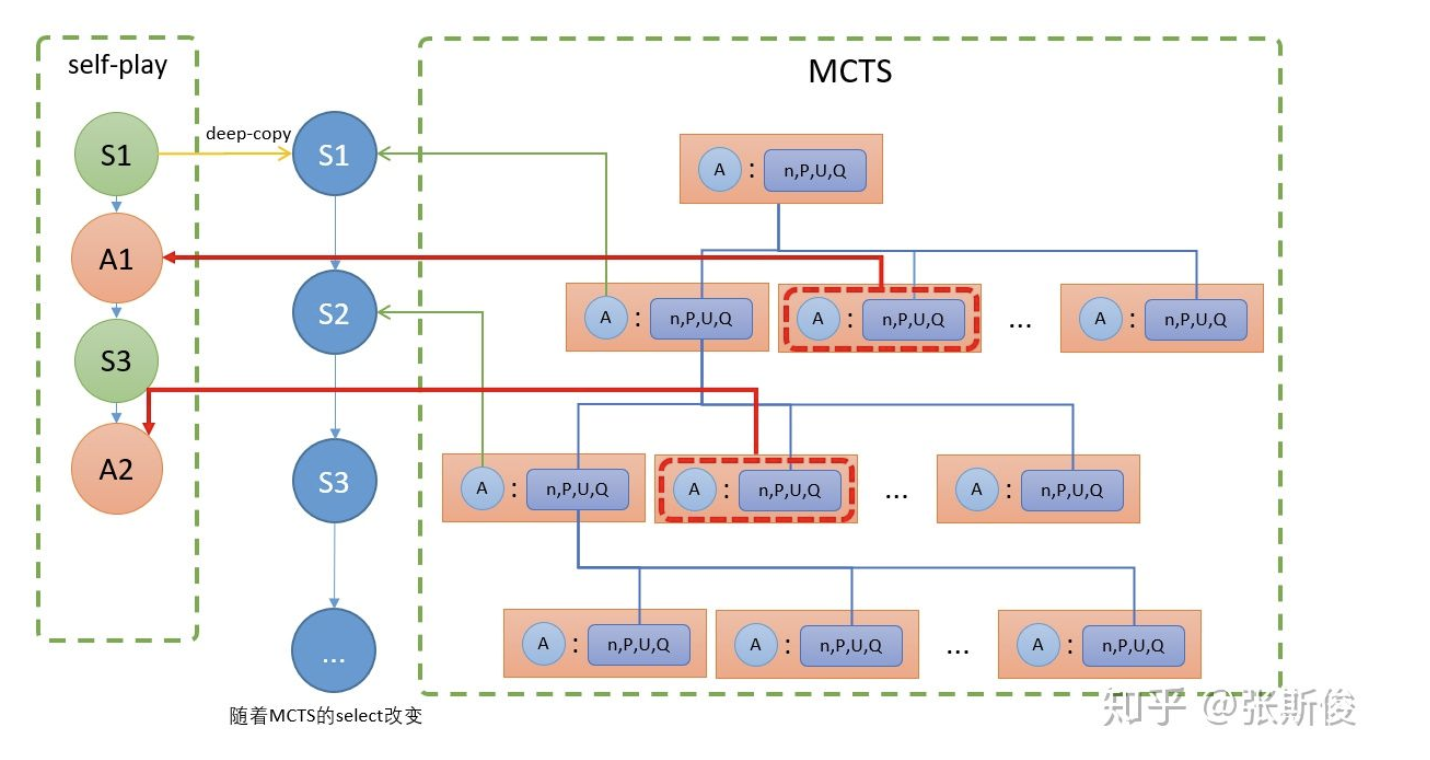
\includegraphics[width=.4\textwidth]{fig/ReinforcementLearning/AlphaZero_Framework.png}
\end{figure}

我们来看看start\_self\_play,开始一场自我对弈:
\begin{python}
def start_self_play(self, player, is_shown=0, temp=1e-3):
        self.board.init_board()
        p1, p2 = self.board.players
        states, mcts_probs, current_players = [], [], []

        while True:
            # ======通过get_action,把当前state放入,预测move和概率的列表
            move, move_probs = player.get_action(self.board,
                                                 temp=temp,
                                                 return_prob=1)

            # ======存储s,move_probs,player
            states.append(self.board.current_state())
            mcts_probs.append(move_probs)
            current_players.append(self.board.current_player)

            # ======执行动作
            self.board.do_move(move)
            if is_shown:
                self.graphic(self.board, p1, p2)

            # ======是否结束
            end, winner = self.board.game_end()
            if end:
                winners_z = np.zeros(len(current_players))
                if winner != -1:
                    winners_z[np.array(current_players) == winner] = 1.0
                    winners_z[np.array(current_players) != winner] = -1.0

                # 重置玩家
                player.reset_player()

                #show文字
                if is_shown:
                    if winner != -1:
                        print("Game end. Winner is player:", winner)
                    else:
                        print("Game end. Tie")
                return winner, zip(states, mcts_probs, winners_z)
\end{python}

这里的关键是get\_action函数,通过这个函数,我们可以调用很多不同的算法,例如随机,纯MCTS算法等进行对弈,这样比较不同算法的质量。但由于我们现在在训练,所以我们需要调用MCTS

在get\_action中,我们调用了mcts.get\_move\_probs,也就是开始用MCTS获得action:
\begin{python}
def get_move_probs(self, state, temp=1e-3):
    for n in range(self._n_playout):
        state_copy = copy.deepcopy(state)
        self._playout(state_copy)
\end{python}

从示例代码中我们能看到,我们会把当前的state用deepcopy进行备份,从这个state\_copy开始建立MCTS。

\_n\_playout表示更新多少次MCTS。具体来说,每进行select-expand-update,就算一次。

\_playout就是建立MCTS的过程,我们就不再重复了。

需要注意两点:
\begin{itemize}
\setlength{\itemsep}{0pt}
\setlength{\parsep}{0pt}
\setlength{\parskip}{0pt}
    \item MCTS的select,是通过max(Q+U),但最终选取的动作是n\_visit最多的动作。这个之前已经讲过,这里只作为提醒。
    \item MCTS只有在自我对弈(selfplay)后,才会进行销毁。啰嗦一句:就是在\_n\_playout轮 playout之后,是保存下来的。 在通过MCTS选择了某个动作后,这个动作节点将会变成根节点,大家可以留意,在get\_action函数的后半部分,都调用了update\_with\_move。
\end{itemize}

\begin{python}
def update_with_move(self, last_move):
    # 重置根节点
    if last_move in self._root._children:
        self._root = self._root._children[last_move]
        self._root._parent = None
    # 输入-1,重置整棵树
    else:
        self._root = TreeNode(None, 1.0)
\end{python}

\subsection{具体例子}
21点、斗兽棋的例子:
\url{https://github.com/louisnino/RLcode/tree/master/Alpha-Zero}

五子棋的例子:
\url{https://github.com/junxiaosong/AlphaZero_Gomoku}

\subsection{斗兽棋的例子解析}
这是个带有点试验性质的游戏,因为在棋盘上包含一些对双方都一样的随机性。

规则:
\begin{itemize}
\setlength{\itemsep}{0pt}
\setlength{\parsep}{0pt}
\setlength{\parskip}{0pt}
    \item 双方棋子包括象、狮、虎、豹、狼、狗、猫、鼠8个棋子,分布在4x4大小的棋盘上;
    \item 关键:棋子在开始的时候,是盖上的,双方需要通过翻棋才能知道棋子是什么,也只有棋子被翻开才能移动;
    \item 象吃狮,狮吃虎,虎吃豹,豹吃狼,狼吃狗、狗吃猫、猫吃鼠、鼠吃象。最终全部棋子被吃完的失败;
\end{itemize}


%\printbibliography
\bibliography{../ref}
\bibliographystyle{IEEEtran}
\end{document}